\chapter{Introducción Específica}

\label{Capitulo2}

En este capítulo se desglosan las diferentes herramientas tanto de hardware como software, elegidas para el desarrollo del robot propuesto.

\section{Robot Operating System}

Típicamente denominado ROS, es un framework de robótica de código abierto, el cual fue diseñado originalmente para robots de uso académico. Sin embargo, al día de hoy su uso se ha extendido tanto a la industria como al público aficionado.\newline
ROS ofrece un variado set de herramientas que facilitan las tareas del roboticista en tareas tales como paso de mensajes, computación distribuida e implementación de algoritmos para aplicaciones robóticas.

\subsection{Organización de archivos}

Es adecuado considerar a ROS como algo más que un framework de desarrollo y referirnos a el como un meta-sistema-operativo, ya que ofrece no solo herramientas y librerías sino también funciones similares a las de un sistema operativo. Entre ellas, podemos citar su abstracción del hardware, manejo de paquetes y un completo \textit{toolchain} de compilación. Así también, tal como en un sistema operativo ``real'', los archivos que componen ROS se encuentran organizados en el disco duro de una manera particular, la cual se expresa en la figura \ref{fig:rosSistemaDeArchivos}.

\begin{figure}[ht]
    \centering
    \def\svgwidth{350pt}
    \input{./Figures/estructura_archivos_ros.pdf_tex}
    \caption{Organización de archivos en ROS}
    \label{fig:rosSistemaDeArchivos}
\end{figure}

\newpage
A continuación se detalla en qué consiste cada uno de los bloques que la componen:
\begin{itemize}
    \item \textbf{Paquetes}: Los paquetes de ROS representan la unidad básica de sofware en la plataforma. Estos contienen uno o mas programas de ROS (nodos), librerías, archivos de configuración, etc, los cuales son organizados como una unidad coherente.
    \item \textbf{Manifiesto del paquete}: Esta representado por un archivo único dentro del paquete y el mismo contiene información sobre el mismo tal como el nombre, autor, tipo de licencia, dependencias, banderas de compilación, etc. El archivo \file{package.xml} encontrado en la raíz del paquete es el manifiesto del mismo.
    \item \textbf{Metapaquete}: Es un paquete que hace referencia a uno o mas paquetes usualmente relacionados entre sí, pero sin estar necesariamente acoplados fuertemente unos con otros. El software proveído con este proyecto es un metapaquete.
    \item \textbf{Manifiesto del metapaquete}: Similar al manifiesto del paquete, con la diferencia que el mismo puede incluir dependencias a de tiempo de ejecución hacia otros paquetes.
    \item \textbf{Mensajes}: Representados con la extensión \file{.msg}, son los tipos de datos utilizados por ROS internamente para comunicar los distintos procesos entre sí. El usuario puede definir tipos de mensajes personalizados con campos adaptados a sus necesidades en del directorio \file{msg} dentro del paquete.
    \item  \textbf{Servicios}: Representados con la extensión \file{.srv}, representan interacciones del tipo solicitud/respuesta entre distintos procesos. Los formatos tanto para solicitud como para respuesta pueden definirse en el directorio \file{srv} dentro del paquete.
    \item \textbf{Repositorios}: La gran mayoría de los paquetes de ROS son mantenidos utilizando un sistema de control de versiones (SCV) tales como Git, Mercurial o SVN. Es común encontrar metapaquetes definidos dentro de un mismo único repositorio, el cual es el caso para el repositorio proveído en este trabajo.
\end{itemize}

\subsection{Arquitectura interna}
ROS esta construido sobre una arquitectura basada en grafos, esto significa que las tareas de cómputo son realizadas a través de una red de procesos llamados nodos. Esta red es denominada \textit{Computation Graph} o grafo de cómputo.\newline
Los principales componentes de este grafo son los nodos, el \textit{master} o maestro, el \textit{parameter server} o servidor de parámetros, además de los mensajes, tópicos, servicios y \textit{bags} o bolsas. Cada uno de estos elementos contribuye al funcionamiento del Computation Graph con una funcionalidad específica. Los elementos que lo componen, mostrados en la figura \ref{fig:computationGraph}, se describen a continuación:

\newpage

\begin{figure}[ht]
    \centering
    \def\svgwidth{350pt}
    \input{./Figures/ros_computation_graph.pdf_tex}
    \caption{Estructura del \textit{Computation Graph} de ROS}
    \label{fig:computationGraph}
\end{figure}

\begin{itemize}
    \item \textbf{Nodos}: Son los procesos que realizan las tareas de cómputo dentro del robot, los cuales pueden comunicarse unos con otros a través de la API de ROS. Esto resulta particularmente útil cuando distintos nodos necesitan compartir información entre si. En ROS se fomenta el uso de múltiples nodos que realicen procesos sencillos por sobre procesos grandes y complejos que abarquen toda la funcionalidad.
    \item \textbf{Master}: El ROS Master se encarga de buscar y registrar los diferentes componentes que interactúan en el sisteam. Esto posibilita que diferentes nodos sean capaces de ``encontrarse'' mutuamente, intercambiar mensajes o invocar servicios. En un sistema distribuido, el master debe ejecutarse solamente en una de las computadoras.
    \item \textbf{Servidor de parámetros}: El servidor de parámetros o \textit{parameter server}, permite mantener la información utilizada en configuración de los nodos almacenada en una ubicación central. Esto permite a cada uno de los nodos a acceder y modificar dichos valores.
    \item \textbf{Mensajes}: Los nodos se comunican entre si mediante mensajes, estructuras de datos cuyos campos pueden editarse y permiten ser enviados entre si. Existen tipos de mensajes estandares (enteros, flotantes, booleanos, etc.) así como también es posible definir mensajes propios, adaptados a las necesidades de la aplicación.
    \item \textbf{Tópicos}: Cada mensaje en ROS es transportado utilizando buses llamados tópicos. Cuando un nodo envía un mensaje a través de un tópico, se puede decir que el nodo esta ``publicando un tópico''. Así mismo cuando un nodo recibe un mensaje a través de un tópico, se puede decir que el nodo esta ``subscripto al tópico''. El nodo publicante y el suscriptor no tienen información sobre su mutua existencia, por lo que es posible que existan nodos publicando a tópicos sin suscriptores o viceversa, nodos suscriptos a tópicos sin publicantes.
    \item \textbf{Servicios}: En determinadas aplicaciones, el mecanismo de publicador/suscriptor definido en el ítem anterior podría no ser adecuado. Por ejemplo, en ciertos casos es necesaria una interacción del tipo solicitud/respuesta. En dichas situaciones un nodo podría solicitar la ejecución de un procedimiento rápido por parte de otro nodo y el envío de una respesta con el resultado de dicho cálculo.
    \item \textbf{Logging}: ROS provee un sistema de registro o \textit{logging} denominada Rosbag (bolsa), la cual se utiliza para almacenar información publicada en los tópicos activos, como por ejemplo la proveniente de un sensor que podría ser difícil de generar una y otra vez, pero que a su vez resulta necesaria para depurar determinados algoritmos. Un rosbag permitiría en este caso, generar la información una única vez para luego reproducirla como si fuese una grabación las veces que resulte necesaria.
\end{itemize}

\subsection{Herramienta RViz}

La herramienta RViz (o ROS Visualization tool), es la herramienta oficial de visualización ROS, la cual permite representar de manera gráfica la información transmitida a través de los distintos tópicos. Posee soporte nativo para la mayoría de los mensajes estándar y permite además, expandir su funcionamiento mediante \textit{plugins} los que posiblitan visualizar mensajes personalizados, entre otros.\newline
RViz permite visualizar la representación física del robot, de modo a analizar su configuración de articulaciones (o \textit{joints}) y enlaces (o \textit{links}), como se muestra en la figura \ref{fig:rviz}.

\begin{figure}[ht]
	\centering
	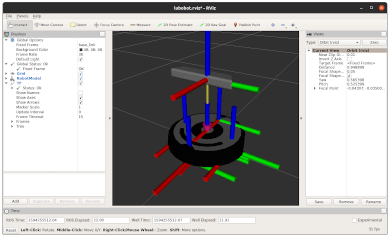
\includegraphics{./Figures/rviz.png}
	\caption{Interfaz gráfica de RViz mostrando los links y joints del robot Lubobot.}
	\label{fig:rviz}
\end{figure}

\subsection{Formato universal de descripción de robots URDF}

El formato universal de descripción de robots o \textit{Universal Robot Description System}, comúnmente referido como URDF es un formato estándar para representación de modelos conformados por múltiples piezas conectadas entre sí, como es el caso de brazos robóticos o líneas de ensamblaje. El mismo es ampliamente utilizado dentro del ecosistema de ROS, plataforma donde vio su origen aunque al día de hoy su uso se ha extendido a herramientas fuera del mismo como MATLAB, la cual permite importar archivos URDF directamente a su \textit{toolbox} de robótica.

\subsection{Librería rosserial}

Es un protocolo para la transmisión serial de mensajes y multiplexación de múltiples tópicos y servicios de ROS sobre un \textit{character device} tal como un puerto UART o un sócket de red.
Además de la definición del protocolo de serialización en si mismo, rosserial se compone de otros dos elementos principales:
\begin{itemize}
    \item \textbf{Librerías cliente}: permiten la integración de nodos ROS en diferentes plataformas, apuntando principalmente a sistemas embebidos. Dichas librerias son especializaciones de una clase base, escrita en ANSI C++ para mayor compatiblidad y denominada rosserial\_client. Para este trabajo se realizó un \textit{port} de dicha librería a la plataforma STM32CubeHAL.
    \item \textbf{Interfaz con ROS}: Las librerías cliente requieren de un nodo corriendo en la computadora \textit{host} que funcione como puente entre el serie y la red de ROS, encargándose de des-serializar y serializar los mensajes que llegan y se despachan, respectivamente. La participación de los distintos actores involucrados en el uso de rosserial se muestran en la figura \ref{fig:rosserial}.
\end{itemize}

\begin{figure}[ht]
	\centering
	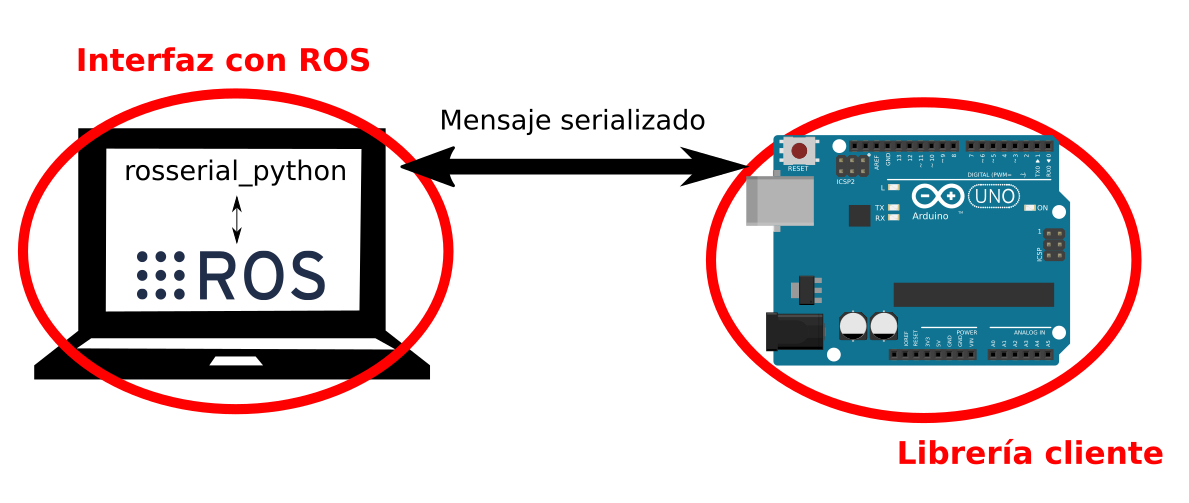
\includegraphics[scale=0.6]{./Figures/rosserial.png}
	\caption{Interacción entre ROS y rosserial corriendo en un microcontrolador}
	\label{fig:rosserial}
\end{figure}

\subsection{Paquete de navegación ros\_navigation\_stack}

El paquete de navegación de ROS, usualmente referido como \textit{navigation stack}, es un set de algoritmos que hacen uso de los sensores del robot y la odometría para permitir controlar al robot utilizando un mensaje estándar mientras el mismo se encarga de evitar choques o atascos sin perder su ubicación en el mapa, previamente generado y proveido al mismo.\newline
Para que un robot pueda hacer uso de este paquete correctamente, es necesario que se satisfaga una serie de requisitos:
\begin{itemize}
    \item Solo puede utilizarse en robots con ruedas en configuración de tracción diferencial u holonómica. Cabe mencionar que el robot presentado en este trabajo es de configuración diferencial.
    \item Es necesario que el robot publique la información sobre las relaciones entre las posiciones de todas las articulaciones y sensores que lo componen.
    \item El robot deberá reportar sus velocidades lineal y angular utilizando un mensaje estándar de ROS.
    \item Un sensor del tipo LIDaR 2D deberá estar presente en el robot para generar el mapa y para el proceso de localización. Alternativamente, es posible utilizar otros tipos de sensores como cámaras de profundidad o \textit{depth cameras} o SONAR, siempre y cuando la información recolectada se publique con el tipo de mensaje adecuado.
\end{itemize}

En la figura \ref{fig:navigationStack} se puede apreciar como se encuentra organizado el paquete de navegación, el cual utiliza dos mapas de obstáculos, uno local y otro global, que son construidos a partir de la información generada por el escaner laser en conjunto con el sistema de navegación. El mapa global es un mapa más extenso en dimiensiones y esta diseñado para el cálculo de trayectorias global, por otro lado, el mapa local es usualmente un mapa mas acotado pero con mayor detalle y su objetivo es el de evadir obstáculos cercanos.

\begin{figure}[ht]
    \centering
    \def\svgwidth{350pt}
    \input{./Figures/navigation_stack.pdf_tex}
    \caption{Configuración típica del paquete de navegación en ROS}
    \label{fig:navigationStack}
\end{figure}

Los mapas global y local son utilizados por los planeadores global y local, respectivamente. El planeador global se encarga de generar un plan para ir de un punto a otro del mapa homónimo. Por otro lado, el local se encarga de controlar los distintos actuadores del robot, por ejemplo las ruedas, para llevar a cabo el plan global pero a la vez que esquiva los obstaculos cercanos que puedan aparecer, incluso si los mismos no se encontrasen registrados en el mapa global. Esto resulta especialmente útil a la hora de esquivar obstáculos nuevos, hasta el momento desconocidos.

\section{iRobot Roomba 500}

El Roomba es un robot de limpieza fabricado y comercializado por la compañía iRobot. El primer modelo salió al mercado en el año 2002 y ha recibido siete actualizaciones desde entonces. En cada iteración, se han mejorado aspectos tanto de diseño como funcionalidad y esto le ha permitido mantenerse como el robot de limpieza con mas unidades vendidas en el mundo.\newline
Todos los Roomba incluyen una serie de sensores táctiles, ópticos y acústicos que le permiten detectar obstáculos, residuos, así como escalones o desniveles en el piso.\newline
A nivel de locomoción, se catalogan como robots móviles con ruedas y utilizan el tipo de tracción diferencial, el cual consiste en dos ruedas motrices independientes que le permiten ejecutar giros de 360 grados. Esto es posible sin que el robot deba incurrir en desplazamiento lineal alguno como en el caso de los automóviles, por citar un ejemplo.\newline
La base móvil utilizada para este trabajo consiste en un Roomba de la serie 500 como el mostrado en la figura \ref{fig:roomba}, el cual fue introducido al mercado en el año 2007 y se mantuvo en el mercado hasta el 2017. Actualmente es posible conseguir estos equipos en condicion de usado o remanufacturado a precios muy accesibles comparado al precio de un equipo mas actual.

\begin{figure}[ht]
	\centering
	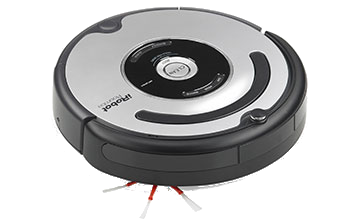
\includegraphics[scale=2.5]{./Figures/roomba.png}
	\caption{iRobot Roomba 500, utilizado como base móvil para este trabajo.\protect\footnotemark}
	\label{fig:roomba}
\end{figure}

\footnotetext{\url{https://uncrate.com/assets_c/2009/04/roomba-560-stretched-thumb-960x640-3177.jpg}}

\subsection{Roomba Open Interface}
Todos los Roomba lanzados a partir del año 2005 son compatibles con una interfaz de comunicación serial denominada Roomba Open Interface, a la cual es posible acceder mediante la conexión a un puerto físico disponible en la placa madre del robot. Esto habilita al usuario a todo tipo de interacción con el hardware del robot, tales como consultar la lectura de cada uno de sus sensores, así como comandar sus actuadores. Este protocolo ha sido actualizado a la par de de las sucesivas actualizaciones del Roomba para ofrecer nuevas funcionalidades o mejoras y en cada caso, se encuentra acompañado de un documento oficial por parte de iRobot en formato PDF\protect\footnotemark.

\footnotetext{\url{https://cdn-shop.adafruit.com/datasheets/create_2_Open_Interface_Spec.pdf}}

\section{Placa de desarrollo STM32-NUCLEO}

Es una familia de placas de desarrollo elaboradas por la compañía ST. Entre sus características principales se destacan:

\begin{itemize}
    \item Bajo costo
    \item Compatibilidad con \textit{shields} de Arduino
    \item Programador/debugger ST-Link integrado
    \item Librería del tipo HAL con variados ejemplos de código
\end{itemize}

De modo a garantizar la escalabilidad del sistema, para este proyecto se optó por una de las placas mas avanzadas de esta familia, denominada NUCLEO-F746ZG y mostrada en la figura \ref{fig:stm32nucleo}. La misma provee un microcontrolador ARM Cortex-M7 con FPU de doble precisión, 320 kB de RAM, así como 1 MB de Flash. Ofrece además conexión ethernet y una amplia cantidad de GPIOs.

\begin{figure}[ht]
	\centering
	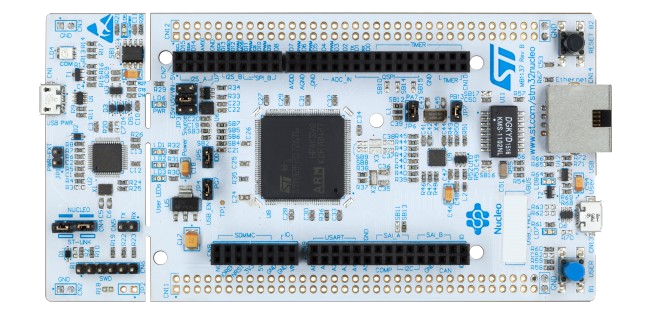
\includegraphics[scale=1.5]{./Figures/stm32nucleo.png}
	\caption{Placa de desarrollo STM32 NUCLEO-F746ZG elegida para comandar el robot.\protect\footnotemark}
	\label{fig:stm32nucleo}
\end{figure}

\footnotetext{\url{https://www.carminenoviello.com/wp-content/uploads/2015/12/nucleo_144_large-2-660x330.jpg}}

\section{Sensor Kinect 360}
\subsection{Descripción}
\subsection{Comparación con otras cámaras de profundidad}
\section{Unidad de medición inercial MPU6050}
\subsection{Descripción}
\subsection{Comparación con otras IMU}
